\chapter{Benutzeroberfläche(UI)}
\section{Konzeption}
Während der Entwicklung wurde ein einfaches Frontend zu Testzwecken angelegt. 
Deshalb soll nun ein Plan entwickelt werden, wie die Benutzeroberfläche aussehen soll und welche Funktionen sie bieten soll:
\begin{center}
  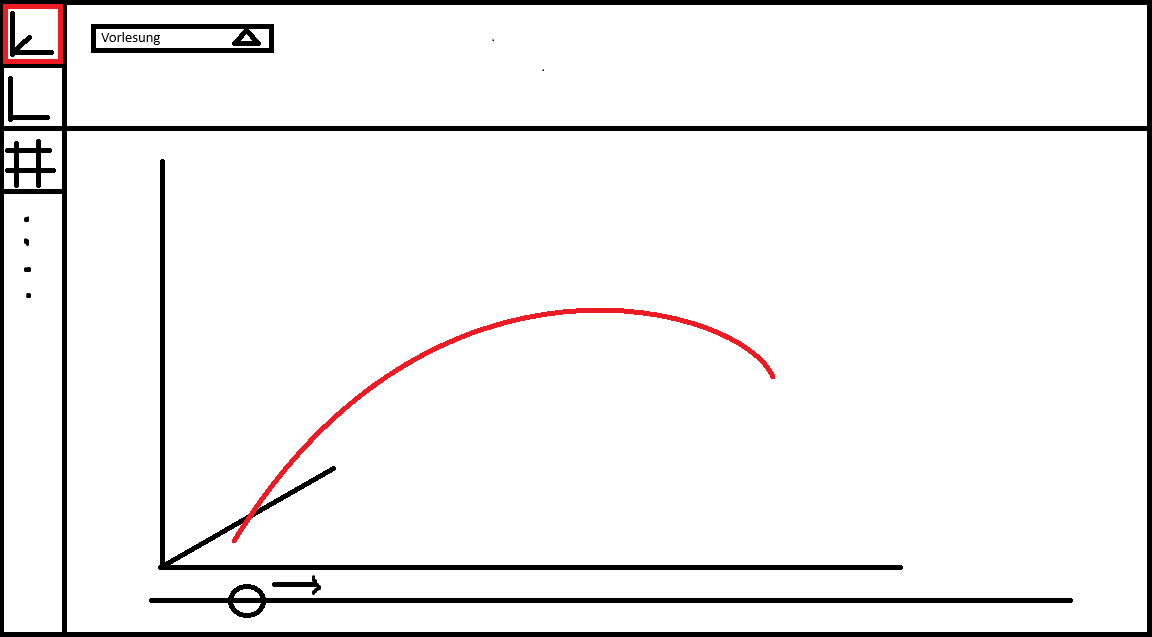
\includegraphics[width=1\textwidth]{../images/UI/SkizzeUI.png}
\end{center}
In dieser Skizze wurden die Grundfunktionen der Benutzeroberfläche festgelegt und die Anordnung der einzelnen Elemente skizziert.
Über eine Navbar an der linken Seite kann zwischen den einzelnen Seiten gewechselt werden. 
Auf der Hauptseite wird eine Heatmap angezeigt, die die Lautstärkeverteiung im Vorlesungsraum räumlich darstellt, wobei mit einem Dropdown-Menü der anzuzueigende Zeitraum ausgewählt werden kann.
Durch den ausgewählten Zeitraum kann anschließend mit einem Schieberegler die Zeit ausgewählt werden, für die die Lautstärke angezeigt werden soll.
Im nächsten Nav-Item sollen die einzelnen 2D-Grafen der jeweiligen Sensoren angezeigt werden. 
Das dritte Nav-Item soll einen tabellarischen Überblick über die gesammelten Daten geben, die in der Datenbank gespeichert sind.
Die Nvabar bietet Raum für zukünfitge Erweiterungen.
